\outlineSubframe{Korrektheit eines Algorithmus}

\begin{frame}{Korrektheit von Algorithmen}{Allgemeines (Vgl. \cite{wiki:algo})}
    \begin{itemize}[<+->]
        \item Jeder Algorithmus sollte auch in allen Fällen das korrekte Ergebnis liefern...
        \item Klingt simpel, aber eindeutiger Beweis für alle Eingaben oft schwierig
        \item Testen an ausgewählten Beispielen \textbf{nicht} ausreichend
        \begin{itemize}
            \item Jedoch verringern umfangreiche Tests natürlich das Risiko eines unentdeckten Fehler
        \end{itemize}
        \item Korrektheit lässt sich im Grunde nur durch formalen Beweis zeigen
        \begin{itemize}
            \item Wie zum Beispiel Induktionsbeweis
            \item Diese sind häufig sehr umfangreich und komplex...
            \item ...und deshalb auch nicht Teil der Vorlesung
        \end{itemize}
    \end{itemize}
\end{frame}

\begin{frame}{Korrektheit von Algorithmen}{}
\begin{minipage}{0.4\textwidth}
            \begin{figure}
                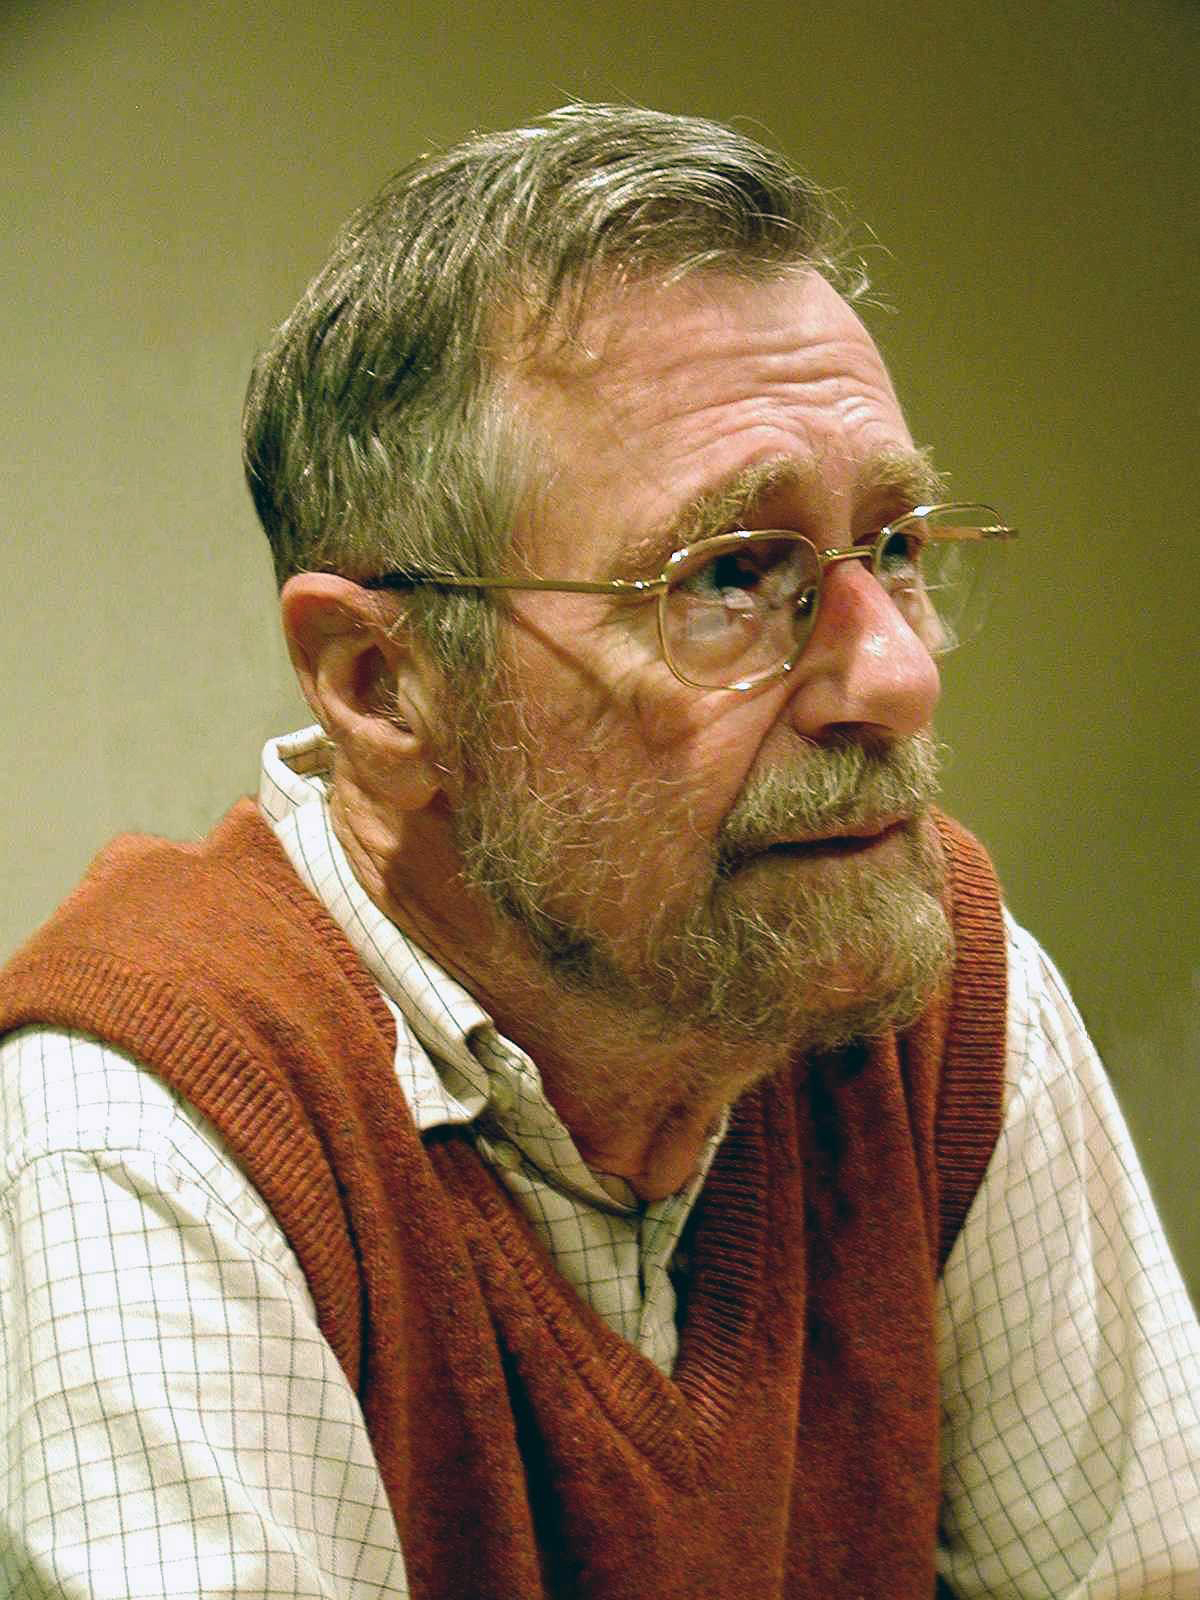
\includegraphics[height=4.5cm]{graph/dijkstra}
                \caption*{Quelle: \cite{wiki:dijkstra}}
            \end{figure}
        \end{minipage}
        \hfill
        \begin{minipage}{0.55\textwidth}
            \textit{„Program testing can be used to show the presence of bugs, but never to show their absence!.“} \\\\Edsger W. Dijkstra
        \end{minipage}
\end{frame}

\outlineSubframe{Komplexitätsanalyse}

\begin{frame}{Speicherkomplexität}{Wie lässt sich diese messen?}
    \begin{itemize}[<+->]
        \item Wie schon erwähnt: Der verbrauchte Speicher ist Sprach- und Rechnerabhängig
        \item Mögliche Lösung über Definition von Referenzsprache und -system
        \item Messungen sind allerdings nicht repräsentativ
        \item Deswegen wird in der formalen Informatik mit dem \textit{Random-Access-Machine}(RAM) Modell gearbeiteet
        \begin{itemize}
            \item Besteht im Grunde ausabzählbar unendlich vielen addressierbaren Speicherzellen
            \item Für einen Algorithmus wird dann bestimmt, wie viele Speicherzellen genutzt werden müssen
            \item Dies entspricht dann der Speicherkomplexität
        \end{itemize}
    \end{itemize}
\end{frame}

\begin{frame}{Laufzeitkomplexität}{Grundlegendes}
    \begin{itemize}[<+->]
        \item Gleiches Problem wie bei der Speicherkomplexität
        \item Deswegen hier ähnliches Modell:
        \begin{itemize}
            \item Man bestimmt die Anzahl von "`atomaren Operationen"' des Algorithmus
            \item Diese Operationen sind vergleichbar mit Assembler-Befehlsrepertoire
        \end{itemize}
        \item Beispiele für atomare Operationen:
        \begin{itemize}
            \item Addition/Subtraktion/Multiplikation/Division zweier Zahlen
            \item Lesen einer Variable von einer Speicheradresse
            \item Schreiben einer Variable an eine bestimmte Adresse
            \item Random Access in Arrays
            \item Vergleich zweier Zahlen
        \end{itemize}
    \end{itemize}
\end{frame}

\begin{frame}[fragile]{Beispiel einer Komplexitätsanalyse}{Vertauschen zweier Zahlen I}
\lstset{style=java}
\begin{lstlisting}
public void swap(int first, int second){
    int tmp = first;
    first = second;
    second = first;
}
\end{lstlisting}

\begin{itemize}
    \item Laufzeitkomplexität: \visible<2->{$O(3)$}
    \item<3-> Speicherkomplexität(In Byte): \visible<4->{$O(12)$}
\end{itemize}
\end{frame}

\begin{frame}[fragile]{Beispiel einer Komplexitätsanalyse}{Vertauschen zweier Zahlen II}
\lstset{style=java}
\begin{lstlisting}
public void swap(int first, int second){
    first = first + second;
    second = first - second;
    first = first - second;
}
\end{lstlisting}

\begin{itemize}
    \item Laufzeitkomplexität: \visible<2->{$O(6)$}
    \item<3-> Speicherkomplexität(In Byte): \visible<4->{$O(8)$}
\end{itemize}
\end{frame}

\begin{frame}{Probleme und Probleminstanzen}
    \begin{itemize}[<+->]
        \item Komplexität ist selten statisch
        \item In der Regel von Problem und der konkreten \textit{Probleminstanz} abhängig
        \begin{itemize}
            \item Problem: z.B. Das sortieren einer Liste
            \item Probleminstanz: konkrete Liste die sortiert werden soll, z.B. $(7, 3, 12, -5, 45)$
        \end{itemize}
        \item Die Probleminstanz hat meist einen oder mehrere dynamische Faktoren von denen die entgültige Komplexität abhängt
        \begin{itemize}
            \item Für Sortieren: \visible<+->{Länge der Liste}
        \end{itemize}
        \item Angegeben werden in der Komplexität nur noch die skalierenden Faktoren
    \end{itemize}
    
    Vgl. \cite{ottmann2017} S. 3 ff
\end{frame}

\begin{frame}[fragile]{Dynamische Komplexität}{Ein Beispiel}
\lstset{style=java}
\begin{onlyenv}<+|handout:0>
\begin{lstlisting}
//A-> Array mit Elementen, n->Länge von A
int sumList(int[] A, int n){
    int sum = 0;
    for(int i=0;i<n;i++){
        sum+=A[i]
    }
    return sum;
}
\end{lstlisting}
\end{onlyenv}

\begin{onlyenv}<+->
\begin{lstlisting}
//A-> Array mit Elementen, n->Länge von A
int sumList(int[] A, int n){
    int sum = 0;            //Kosten: 1, Anzahl: 1 mal
    for(int i=0;i<n;i++){   //Kosten: 2, Anzahl: n+1 mal
        sum+=A[i]           //Kosten: 2, Anzahl: n mal
    }
    return sum;             //Kosten: 1, Anzahl: 1 mal
}
\end{lstlisting}
\end{onlyenv}


\visible<+->{$ \tau(n) = 1 + 2\cdot(n+1) +  2n + 1 $}

\visible<+->{$ \tau(n) = 1+ 2n + 2 + 2n +1 $}

\visible<+->{$ \tau(n) = 4n + 4 $}
\visible<+->{$ \tau(n) = c_1n+c_2 $}

\visible<+->{$\Rightarrow O(n)$}
\end{frame}